\documentclass{beamer}
\usetheme{Warsaw}
\usepackage[absolute,overlay]{textpos}
\usepackage{graphicx}
\useoutertheme{infolines}
\usecolortheme{seahorse}
\usepackage{caption}
\usepackage{amsfonts}
\setbeamertemplate{caption}[numbered]
\usepackage{amsmath,mathrsfs,amssymb}
\usepackage{geometry}
\usepackage{pgfplots} 
\usepackage{tikz, xifthen}
%\usepackage[french]{algorithm2e}
\usepackage{animate}
\usepackage{hyperref}
%\usepackage[style=authoryear]{biblatex}
%\addbibresource{biblio.bib}
\usepackage{cancel}
\usepackage{soul}
\usetikzlibrary{matrix, positioning, arrows.meta, fit}
\usepackage{fp}
\usepackage{pgfplots}
%\pgfplotsset{compat=1.17}
\usepackage{listings}  % Ajout du package listings
\usepackage{lipsum}    % Pour le texte de remplissage (lipsum)

% Configuration du package listings pour le langage C
\lstdefinestyle{mystyle}{
	belowcaptionskip=1\baselineskip,
	breaklines=true,
	frame=L,
	xleftmargin=3em, % Reduced left margin
	language=C,
	showstringspaces=false,
	basicstyle=\scriptsize\ttfamily, % Smaller font size
	keywordstyle=\color{codekeyword},
	commentstyle=\color{codecomment},
	stringstyle=\color{codestring},
	backgroundcolor=\color{codebg},
	numbers=left,
	numberstyle=\tiny\color{gray},
	stepnumber=1,
	numbersep=10pt, % Reduced number separation
	captionpos=b,
	tabsize=2,
	breakatwhitespace=false,
}

\usepackage{xcolor}

\definecolor{codebg}{RGB}{240,240,240}
\definecolor{codecomment}{RGB}{0,128,0}
\definecolor{codekeyword}{RGB}{0,0,255}
\definecolor{codestring}{RGB}{255,100,0}

\lstdefinestyle{customc}{
	belowcaptionskip=1\baselineskip,
	breaklines=true,
	frame=L,
	xleftmargin=\parindent,
	language=C,
	showstringspaces=false,
	basicstyle=\footnotesize\ttfamily,
	keywordstyle=\bfseries\color{codekeyword},
	commentstyle=\itshape\color{codecomment},
	stringstyle=\color{codestring},
	backgroundcolor=\color{codebg},
	numbers=left,
	numberstyle=\tiny\color{gray},
	stepnumber=1,
	numbersep=10pt,
	captionpos=b,
	tabsize=2,
	breakatwhitespace=false,
}


\setbeamertemplate{footline}{%
	\leavevmode\hbox{%
		\begin{beamercolorbox}[wd=1.581cm,ht=2.5ex,dp=1.125ex,leftskip=.3cm]{author in head/foot}%
			\usebeamerfont{author in head/foot}\insertframenumber/\inserttotalframenumber
		\end{beamercolorbox}%
		\begin{beamercolorbox}[wd=1.0\paperwidth,ht=2.5ex,dp=1.125ex,leftskip=.3cm]{title in head/foot}%
			\usebeamerfont{title in head/foot}\hspace{2.6cm}\insertshorttitle
	\end{beamercolorbox}}%
	\vskip0pt}


\logo{
\includegraphics[height=0.5cm]{logo-embxinp.png}}

% \colorlet{bleu_item}{blue!80!green}
% \setbeamertemplate{itemize item}[square]
% \setbeamercolor{itemize item}{fg=bleu_item}
% \setbeamertemplate{frametitle continuation}{}


\hypersetup{breaklinks=true}
\setbeamercolor{framesource}{fg=gray}
\setbeamerfont{framesource}{size=\tiny}
\newcommand{\source}[1]
{
	\begin{beamercolorbox}[ht=0cm,right]{framesource}
		\usebeamerfont{framesource}\usebeamercolor[fg]{framesource} Source: {#1}
	\end{beamercolorbox}
	\vspace{-6mm}	
}
\newcommand{\e}{\mathrm{e}}
\pdfstringdefDisableCommands{%
	\def\\{}%
	\def\texttt#1{<#1>}%
}

% Title Page
\title{ Resolution of the linear Boltzmann equation by Monte Carlo method}
\subtitle{}

\author{Antoine Boucher\\
	Gabriel Rodiere\\
	Clément Aumonier\\
	Guillaume Doyen\\
	Khaoula El Maddah}
\institute{}
\titlegraphic{
\includegraphics[height=1.8cm]{logo-embxinp.png}}
\date{}
\titlegraphic{
\includegraphics[height=1cm]{logo-embxinp.png}}

% Begin Document
\begin{document}
	
	% Title Page
	\begin{frame}
		\titlepage
	\end{frame}
	
	% Outline Slide
	\begin{frame}
		\frametitle{Table of contents}
		\tableofcontents
	\end{frame}
	
	\section{Introduction}
	\begin{frame}{Boltzmann equation}
		The transport equation in an infinite medium with its corresponding deterministic collisional component can be expressed as:
		\begin{equation*}
			\partial _t u(x,t,\textbf{v}) + \textbf{v} \cdot \nabla u(x,t,\textbf{v}) + v\sigma_t (x,t,\textbf{v})u(x,t,\textbf{v})= v\sigma_s(x,t,\textbf{v})\int P (x,t,\textbf{v},\textbf{v}')u(x,t,\textbf{v}')d\textbf{v}' \label{ref11}
		\end{equation*}
		Where 
		\begin{equation*}
			\sigma_s (x,t,\textbf{v})= \int \sigma_s (x,t,\textbf{v},\textbf{v}')d\textbf{v}', \quad  P (x,t,\textbf{v},\textbf{v}')=
			\frac{\sigma_s (x,t,\textbf{v},\textbf{v}')}{\sigma_s (x,t,\textbf{v})}
		\end{equation*}
		
	\end{frame}
	\section{The existence and uniqueness of the solution}
	\section{Monte Carlo method}
	\begin{frame}{Example a way to calculate $\pi$}
		Let a circle of radius $r = 1$ inscribed in a square of side $2$. When throwing stones in the air and count the number of stones landing within the circle, an estimate of $\pi$ is: 
		\begin{equation*}
			\pi_N =\frac{\text{Number of stones within the circle}}{4 N}
		\end{equation*}
		\begin{figure}[h]
			\centering
			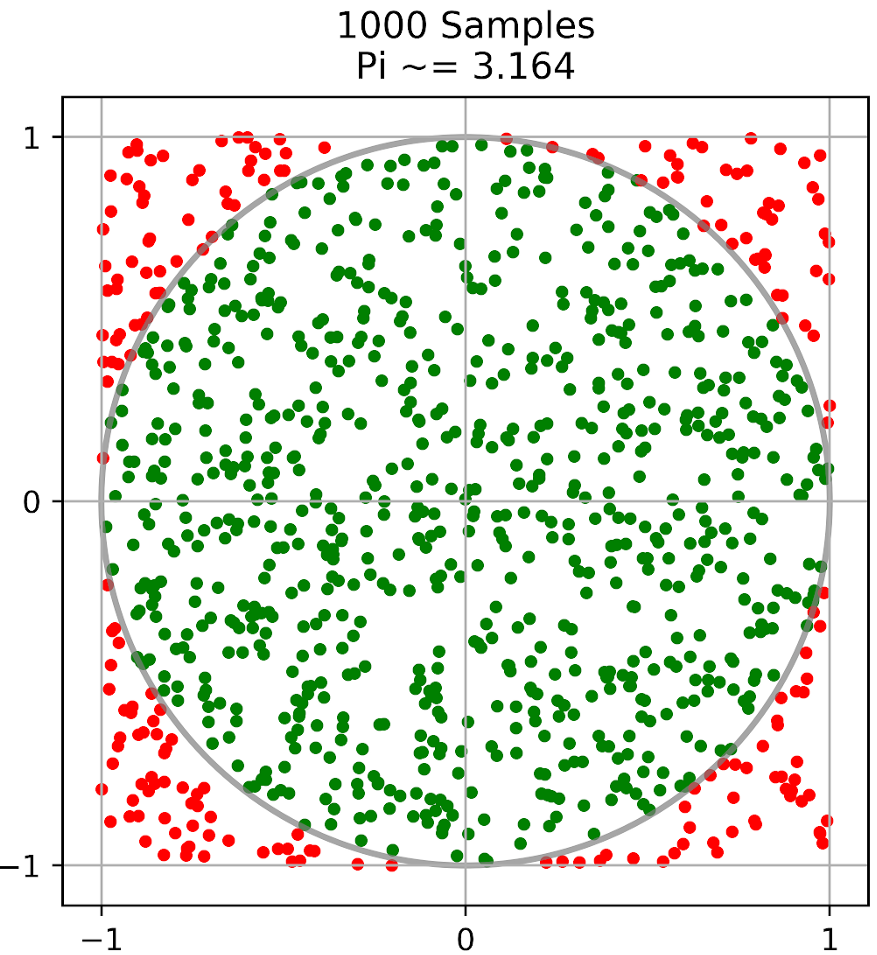
\includegraphics[width=0.5\linewidth]{pi.png}
			\label{fig:votre_label}
		\end{figure}
	\end{frame}
	\section{Resolution of the equation}
	\begin{frame}{Variable change}
		The approach involves a series of variable changes. The initial step is re-expressing the transport equation with respect to a characteristic $x + vt$. As a result, it transforms into:
		\begin{equation*}
			\begin{split}
				\partial _s u(x+\textbf{v}s,s,\textbf{v}) &= -v\sigma_t (x+\textbf{v}s,s,\textbf{v})u(x+\textbf{v}s,s,\textbf{v}) \\
				&\quad + v\sigma_s(x+\textbf{v}s,s,\textbf{v})\int P (x+\textbf{v}s,s,\textbf{v},\textbf{v}')u(x+\textbf{v}s,s,\textbf{v}')d\textbf{v}'
			\end{split}
		\end{equation*}
	\end{frame}
	
	\begin{frame}{Equation Transformation with Multiplication and Integration}
		After multiplying both sides of the equation by:
		\begin{equation*}
			e^{\int _0^s v\sigma_t (x + \textbf{v}\alpha,\alpha, v) d\alpha}
		\end{equation*}
		Following that, we obtain
		\begin{equation*}
			\begin{split}
				&\partial _s [u(x+\textbf{v}s,s,\textbf{v})e^{\int _0^s v\sigma_t (x + \textbf{v}\alpha,\alpha, v) d\alpha}] \\
				&= e^{\int _0^s v\sigma_t (x + \textbf{v}\alpha,\alpha, v) d\alpha} v\sigma_s(x+\textbf{v}s,s,\textbf{v})\int P (x+\textbf{v}s,s,\textbf{v},\textbf{v}')u(x+\textbf{v}s,s,\textbf{v}')d\textbf{v}'
			\end{split}
		\end{equation*}
	\end{frame}
	
	\begin{frame}{Integration of the equation}
		We get after integrating the equation between [0, t]:
		
		\begin{multline*}
			\resizebox{\linewidth}{!}{$
				u(x+\textbf{v}t,t,\textbf{v}) = u_0(x, \textbf{v}) \exp\left(- \int_{0}^{t} v\sigma_t\left(x + \textbf{v} \alpha, \alpha, \textbf{v}\right) d\alpha\right)$} \\
			\resizebox{\linewidth}{!}{$
				+ \int_{0}^{t} \int v\sigma_s\left(x + \textbf{v}s, s, \textbf{v}\right) u\left(x + \textbf{v}s, s, \textbf{v}'\right) e^{- \int_s^t v\sigma_t\left(x + \textbf{v} \alpha, \textbf{v}\right) d\alpha} P\left(x + \textbf{v} s, s, \textbf{v}, \textbf{v}'\right) d\textbf{v}'ds$
			}
		\end{multline*}
		
		After a variable change, we obtain:
		
		\begin{multline*}
			\resizebox{\linewidth}{!}{$
				u(x,t,\textbf{v}) = u_0(x - \textbf{v}t, \textbf{v}) \exp\left(- \int_{0}^{t} v\sigma_t\left(x - \textbf{v}(t - \alpha), \alpha, \textbf{v}\right) d\alpha\right)$} \\
			\resizebox{\linewidth}{!}{$
				+ \int_{0}^{t} \int v\sigma_s\left(x - \textbf{v}(t - s), s, \textbf{v}\right) u\left(x - \textbf{v}(t - s), s, \textbf{v}'\right) e^{- \int_s^t v\sigma_t\left(x - \textbf{v}(t - \alpha), \textbf{v}\right) d\alpha} P\left(x - \textbf{v}(t - s), s, \textbf{v}, \textbf{v}'\right) d\textbf{v}'ds$
			}
		\end{multline*}
	\end{frame}
	
	\begin{frame}{Frame Title}
		We also have:
		\begin{multline*}
			\exp\left(- \int_{0}^{t} v\sigma_t\left(x - \textbf{v}(t - \alpha), \alpha, \textbf{v}\right) d\alpha\right) \\ = \exp\left(- \int_{0}^{t} v\sigma_t\left(x - \textbf{v} \alpha,t- \alpha, \textbf{v}\right) d\alpha\right) \\ = \int _t^\infty  v\sigma_t\left(x - \textbf{v} s,t- s, \textbf{v}\right)
			\exp\left(- \int_{0}^{s} v\sigma_t\left(x - \textbf{v} \alpha,t- \alpha, \textbf{v}\right) d\alpha\right) ds
		\end{multline*}
	\end{frame}
	\begin{frame}{The integral form of the Boltzmann equation}
		Then the integral representation of the transport equation is provided by:
		\resizebox{\linewidth}{!}{
			\begin{minipage}{\linewidth}
				\begin{multline*}
					u(x,t,\textbf{v}) =  \int _t^\infty  u_0(x - \textbf{v}t, \textbf{v}) v\sigma_t\left(x - \textbf{v} s,t- s, \textbf{v}\right) \\
					\exp\left(- \int_{0}^{s} v\sigma_t\left(x - \textbf{v} \alpha,t- \alpha, \textbf{v}\right) d\alpha\right) ds\\
					+ \int_{0}^{t} \int v\sigma_s\left(x - \textbf{v}(t - s), s, \textbf{v}\right) u\left(x - \textbf{v}(t - s), s, \textbf{v}'\right) \\
					e^{- \int_s^t v\sigma_t\left(x - \textbf{v}(t - \alpha), \textbf{v}\right) d\alpha} P\left(x - \textbf{v}(t - s), s, \textbf{v}, \textbf{v}'\right) d\textbf{v}'ds \label{ref13}
				\end{multline*}
			\end{minipage}
		}
	\end{frame}
	\section{The semi-analog MC scheme}
	\begin{frame}{Semi-analog scheme}
		Developing a Monte Carlo scheme involves introducing random variables and their associated probability measure to express the equation as an expectation. The choice of this set of random variables is not unique, leading to different Monte Carlo schemes with distinct properties.\\
		For the semi-analog scheme, we introduce the probability measure of the interaction time: 
		\begin{equation*}
			f_{\tau}(\textbf{x}, t, \textbf{v}, s) ds = 1_{[0,\infty[}(s) \, v\sigma_t(\textbf{x} - \textbf{v}s, t - s, v) e^{-\int_{0}^s v\sigma_t(\textbf{x} - \textbf{v}\alpha, t - \alpha, v) \, d\alpha} ds
		\end{equation*}
		$ \forall (x, t, v) \in D \times [0, T] \times \mathbb{R}^3$\\
		We introduce the specified random variables corresponding to the previously identified probability measures.
		
		\begin{equation*}
			\left\{
			\begin{array}{ll}
				\tau \text{ with probability measure } f_{\tau}(\textbf{x}, t, \textbf{v}) \, ds, \\
				\textbf{V}' \text{ with probability measure } P_{\textbf{V}'}^{s}(\textbf{x}, t, s, \textbf{v}, \textbf{v}') \, dv'
			\end{array}
			\right.
		\end{equation*}
		
		
	\end{frame}
	\begin{frame}{Expression of the solution}
		We found the following expectation value:
		\begin{equation*}
			\begin{split}
				u(x, t, v) = & E\left[1_{[t, \infty[}(\tau)u_0(\textbf{x} - \textbf{v}t, \textbf{v}) \right. \\
				& \left. + 1_{[0, t[}(\tau)\frac{\sigma_s(\textbf{x} - \textbf{v}\tau, t - \tau, v)}{\sigma_t(\textbf{x} - \textbf{v}\tau, t - \tau, v)}u(\textbf{x} - \textbf{v}\tau, t - \tau, \textbf{V}')\right]
			\end{split}
		\end{equation*}
		Essentially, the process of constructing a Monte Carlo scheme is based on searching for solutions of expectation that possess this specific structures:
		\begin{equation*}
			u_p(\textbf{x},t,\textbf{v}) = w_p(t) \delta_x(\textbf{x}_p(t))\delta_\textbf{v}(\textbf{v}_p(t))
		\end{equation*}
		Replacing \(u_p\) in the equation yields:
		
		\begin{cases} 
			w_p(t) = 1_{[0,\infty[}(\tau)w_p(0) + 1_{[0,t[}(\tau) \frac{\sigma_s}{\sigma_t}(x_p(t-\tau),t-\tau,\textbf{v}_p(t-\tau))w_p(t-\tau),\\
			x_p(t) = 1_{[0,\infty[}(\tau)(\textbf{x}_0-\textbf{v}t) + 1_{[0,t[}(\tau)(x_{t-\tau}-\textbf{v}\tau),\\
			v_p(t) = 1_{[0,\infty[}(\tau)\textbf{v} + 1_{[0,t[}(\tau)\textbf{V}'. 
		\end{cases}
	\end{frame}
	
	\section{Numerical result}
	\begin{frame}{Numerical result}
		
	\end{frame}
	
	
\end{document}
